\documentclass{standalone}
\usepackage{pgfplots}
\pgfplotsset{compat=1.16}
\begin{document}
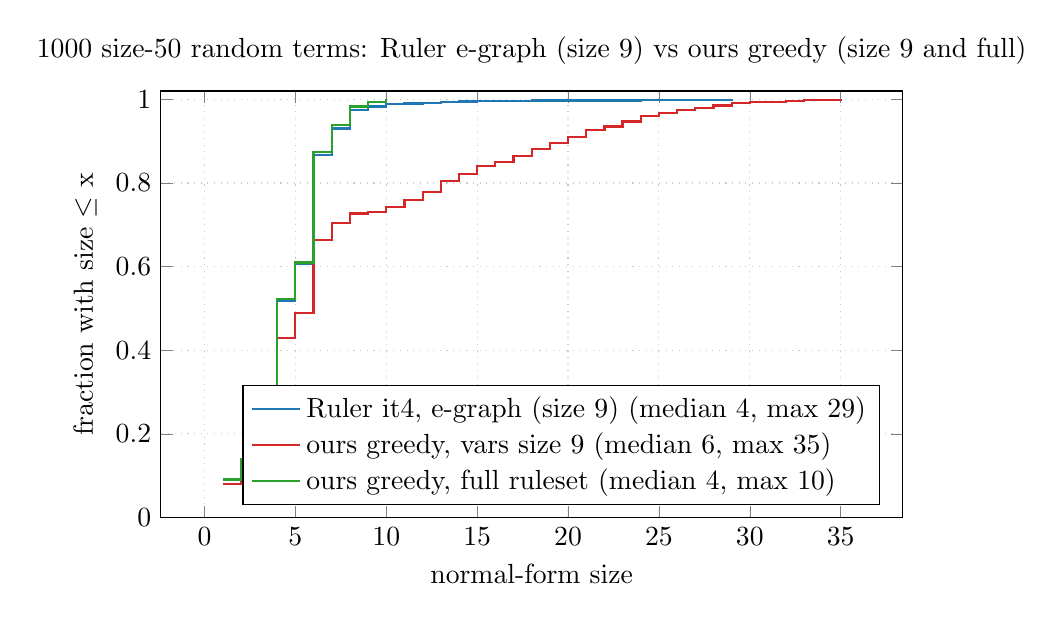
\begin{tikzpicture}
  \begin{axis}[
      width=11cm, height=7cm,
      xlabel={normal-form size}, ylabel={fraction with size $\leq$ x},
      title={1000 size-50 random terms: Ruler e-graph (size 9) vs ours greedy (size 9 and full)},
      ymin=0, ymax=1.02, grid=both, grid style={dotted, gray!40},
      legend pos=south east, legend cell align=left,]
    \definecolor{c0}{HTML}{1f77b4}
    \addplot[color=c0, thick, const plot] coordinates {(1,0.0900) (2,0.1380) (3,0.2910) (4,0.5190) (5,0.6070) (6,0.8670) (7,0.9300) (8,0.9740) (9,0.9830) (10,0.9890) (11,0.9900) (12,0.9910) (13,0.9940) (14,0.9950) (15,0.9960) (18,0.9970) (24,0.9980) (26,0.9990) (29,1.0000)};
    \addlegendentry{Ruler it4, e-graph (size 9) (median 4, max 29)}
    \definecolor{c1}{HTML}{d62728}
    \addplot[color=c1, thick, const plot] coordinates {(1,0.0810) (2,0.1170) (3,0.2410) (4,0.4290) (5,0.4900) (6,0.6630) (7,0.7050) (8,0.7270) (9,0.7310) (10,0.7430) (11,0.7600) (12,0.7780) (13,0.8040) (14,0.8210) (15,0.8410) (16,0.8510) (17,0.8640) (18,0.8820) (19,0.8950) (20,0.9100) (21,0.9260) (22,0.9350) (23,0.9470) (24,0.9610) (25,0.9680) (26,0.9740) (27,0.9790) (28,0.9850) (29,0.9910) (30,0.9930) (32,0.9960) (33,0.9980) (34,0.9990) (35,1.0000)};
    \addlegendentry{ours greedy, vars size 9 (median 6, max 35)}
    \definecolor{c2}{HTML}{2ca02c}
    \addplot[color=c2, thick, const plot] coordinates {(1,0.0910) (2,0.1390) (3,0.2930) (4,0.5220) (5,0.6100) (6,0.8740) (7,0.9380) (8,0.9830) (9,0.9930) (10,1.0000)};
    \addlegendentry{ours greedy, full ruleset (median 4, max 10)}
  \end{axis}
\end{tikzpicture}
\end{document}
